\chapter{Analýza problému}

V této kapitole se pokusíme zjistit, s čím mají začátečníci největší potíže při práci s mikrokontrolery. Prozkoumáme názory studentů FIT ČVUT, kteří absolvovali předmět BI-SAP. Dále se pak podíváme na existující programovou podporu pro vývoj programů pro platformu AVR.

\section{Dotazník}

Na FIT ČVUT se studenti poprvé setkávají s vývojem pro mikrokontrolery nejčastěji v druhém semestru v předmětu BI-SAP. Jsou proto ideálním zdrojem informací o tom, jak začátečníci k programování mikrokontrolerů přistupují, s jakými se setkávají potížemi a co jsou pro ně nejobtížnější překážky k překonání. Prozkoumáme tudíž jejich spokojenost s průběhem výuky pomocí krátkého dotazníku.

Samotný dotazník je velice jednoduchý, ptá se pouze zda respondent souhlasí s následujícími tvrzeními:

\begin{enumerate}
	\item Assembly mi dělalo potíže.
	\item Nemohl jsem dělat úkoly doma / bez přípravku.
	\item Vyvíjet pro AVR nešlo na macOS / Linuxu.
	\item Programy nešlo dobře ladit.
	\item AVR je příliš komplikovaná platforma.
\end{enumerate}

Původním plánem bylo nechat dotazník zveřejněný, dokud nenasbíráme alespoň 100 respondentů. V poměrně krátkém časovém intervalu jednoho dne jsme získali 110 odpovědí a jejich sběr jsme proto ukončili. Ručně jsme protřídili odpovědi, které nebyly validní a zůstalo nám 95 odpovědí. Výsledek dotazníku je poté uveden v grafu na obrázku \ref{fig:survey}.

\begin{figure}
\begin{center}
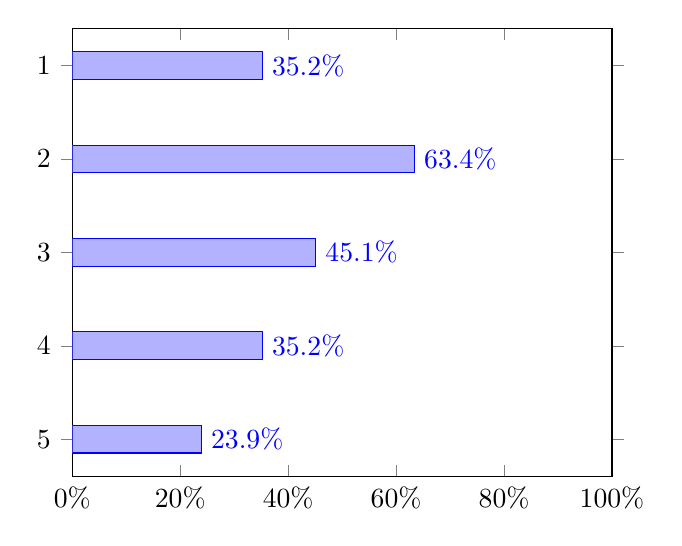
\begin{tikzpicture}
\begin{axis}[
	xbar,
	xmin=0,
	xmax=100,
	xticklabel={\pgfmathparse{\tick}\pgfmathprintnumber{\pgfmathresult}\%},
	symbolic y coords={5,4,3,2,1},
	ytick=data,
	nodes near coords={\pgfmathprintnumber\pgfplotspointmeta\%},
	]
	\addplot coordinates {
		(23.9,5)
        (35.2,4)
        (45.1,3)
		(63.4,2)
		(35.2,1)
		};
\end{axis}
\end{tikzpicture}
\caption{Procenta kladných odpovědí na otázky mezi respondenty}
\label{fig:survey}
\end{center}
\end{figure}

Z odpovědí je nejenom patrné, že je problematické samotné programování v jazyce symbolických adres, ale že jednoznačně největším problémem je závislost na fyzickém přípravku, který musí studenti mít, aby mohli plnit úlohy. Dále se pak jako problém ukázala také nízká kvalita programové podpory pro vývoj pro platformu AVR.

\section{Současný stav řešení}

Aplikací, která se v současné době na FIT ČVUT používá při výuce předmětu BI-SAP\todocite, je AVR studio (konkrétně verze 4). Jedná se o kompletní vývojovou sadu přímo od společnosti Atmel\todocite. Aplikace je však kompatibilní pouze se systémem Microsoft Windows\todocite, je ji proto těžké nebo nemožné zprovoznit na alternativních operačních systémech. To je pro některé uživatele zásadní problém a aplikace proto není kompletním řešením.

Nejpřímočařejším řešením vývoje pro platformu AVR je manuální překlad a nahrávání programu do zařízení. Z našeho oblíbeného jazyka vyprodukujeme patřičným překladačem binární soubor, který poté slinkujeme a nahrajeme do zařízení pomocí programátoru a aplikace. Toto řešení je pro zkušené uživatele často nejjednoduší, avšak obzvlášť pro začátečníky pracující v operačním systému, ve kterém není užití konzolových aplikací možné nebo jednoduché, je tato cesta takřka nemožná.

Pro platformu AVR existuje několik dalších aplikací, které usnadňují vývoj a nahrávání programu. Ukážeme si z nich dvě -- simavr\todocite a Arduino IDE\todocite.

\todoimage{AVR Studio}

Zajímavým projektem je simavr\todocite. Jedná se o konzolovou aplikaci, která umožňuje emulovat běh různých mikrokontrolerů z rodiny AVR. Poskytuje výbornou integraci s ladícím programem gdb, zpětnou logickou analýzu pomocí souborů ve formátu VCD (Value change dump) a snadnou rozšiřitelnost pomocí externích vizualizačních nástrojů. Díky tomu se jedná o výborný nástroj pro lazení složitějších programů. Kvůli tomu je však aplikace nepřívětivá k uživatelům, kteří nejsou již zkušenými programátory, nebo nemají detailní přehled o platformě AVR. Zároveň není aplikací nijak zprostředkován překlad zdrojového kódu do strojového. Uživatel je tudíž nucen řešit tento problém externím překladačem, jako například AVRA\todocite, nebo Avr-GCC\todocite.

Jednou z aplikací cílené na naprosté začátečníky je Arduino IDE\cite{arduino-ide}. Jedná se o aplikaci usnadňující vývoj pro prototypovací platformu Arduino. Aplikace vyčnívá mezi konkurencí svým simplistickým vzhledem a jednoduchostí používání. V aplikaci se programuje v jazyce C, obohaceném o knihovnu funkcí unsadňující ovládání mikrokontroleru. Překlad a nahrání programu do mikrokontroleru proběhne stiskem tlačítka ``Play''. Aplikace také usnadňuje komunikaci s externím zařízením po sériové lince pomocí zabudované konzole. Nikterak však uživateli neusnazuje lazení běžícího programu a uživatel je tak ponechán napospas chybám, které jako začátečník nevyhnutelně udělá.

Mezi její nevýhody však patří, že se pokouší odstínit své uživatele od příliš mnoha aspektů programování pro mikrokontrolery. Nahrávání i překlad programu probíhá automaticky. Aplikace za uživatele doplní i hlavičkové soubory pro danou platformu. Knihovna funkcí poskytnuta uživateli, ačkoliv usnadňuje vývoj, nereprezentuje dobře operace probíhající ``pod kapotou''. Jedná se proto o znalosti, které jsou nepřenositelné na platformy s Arduinem nekompatibilní.

\imagefigurefull{arduino-ide.png}{Arduino IDE}{1.0}

\section{Požadavky na řešení}

Z uvedených aplikací žádná není ideálním řešením pro naprosté začátečníky, pokusíme se proto navrhnout vlastní. Pokusíme se naši platformu navrhnout co uživatelksy nejpřívětivější, aby s ní mohl pracovat i naprostý začátečník. Zároveň se však pokusíme aby byla dostatečně realistická na to, aby následný přechod k platformě AVR byl co nejjednodušší.